\section{Autovalutazione}
Il gruppo ha utilizzato il metodo MoSCoW per scegliere quali aspetti delle specifiche avessero la maggior priorità ed eventualmente scegliere quali specifiche non implementare.

\noindent Le specifiche prefissate per la categoria \textbf{MUST} erano le seguenti:
\begin{itemize}
    \item \textbf{Modellazione di tutti i sistemi tramite rappresentazioni di Ingegneria del Software}:\newline
    Sono stati realizzati i Diagrammi delle classi del Server, i Diagrammi degli Stati di Client e Server, ed i diagrammi sequenza delle operazioni più corpose (la comunicazione tramite WebSocket). I diagrammi sono stati strutturati in modo da essere robusti e coprire tutti gli scenari possibili.
    \item \textbf{Gestione delle stanze lato Server}:\newline
    Il package \textit{model} contiene tutte le strutture dati usate. I messaggi che il client manda al server modificano le strutture dati contenute in \textit{ModelRepository} e il server notifica senza problemi gli eventi accaduti ai client interessati;
    \item \textbf{Gestione degli stati di gioco lato Server}:\newline
    Gli oggetti \textit{Lobby} in particolare possono trovarsi nello stato \textbf{INSIDE\_LOBBY} quando si attendono giocatori nella hall, \textbf{DRAW} o \textbf{SENTENCE} quando si sta giocando e \textbf{SHOWING\_REPORT} quando si stanno visualizzando i report. Il server cambia gli stati delle Lobby in funziona dei messaggi websocket e allo stato della struttura dati in un dato momento temporale;
    \item \textbf{Creazione di un client Web}:\newline
    Sono state create delle pagine Web a cui è possibile accedere da qualsiasi browser. Il design era stato inizialmente pensato solo per la versione Desktop ma è stato esteso anche alla versione Mobile. Il client riesce a comunicare col Server utilizzando messaggi HTTP e WebSocket.
    \item \textbf{Creazione di Test per verificare il corretto funzionamento del sistema}:
    Tutte le richieste API sono state testate con automatismi. La comunicazione tra server e client tramite WebSocket è stata resa più agevole grazie a strumenti come Redux DevTools. Non sono stati effettuati test con un numero estremamente elevato di client ma sono state giocate più partite in contemporanea anche in condizioni internet abbastanza estreme con risultati più che soddisfacenti.
\end{itemize}

\noindent La specifica prefissata per la categoria \textbf{SHOULD} era la seguente:
\begin{itemize}
    \item \textbf{Creazione di un client Mobile}:\newline
    Oltre ad aver ripensato le pagine del client web in modo da funzionare perfettamente anche sugli schermi più piccoli è stata creata un'app Mobile usando ReactNative. L'applicazione funziona su un elevato numero di dispositivi, l'unico prerequisito è la presenza di una connessione ad internet disponibile.
\end{itemize}

\noindent Le specifiche prefissate per la categoria \textbf{WOULD} erano la seguenti:
\begin{itemize}
    \item \textbf{Implementazione di un sistema di messaggistica}:\newline
    È stata implementata una Chat funzionante tramite l'uso di WebSocket e di un canale apposito. È possibile usare la chat quando si entra in una lobby, mentre si sta giocando e mentre si stanno visualizzando i risultati finali.
        \item \textbf{Possibilità di consultare report di partite passate}:\newline
        Il server permette di recuperare la lista di tutte le partite giocate in passato. È quindi anche possibile scaricare tutti i report relativi ad una determinata partita. È possibile scaricare tutti i report di una partita a cui si è presa parte, non solo i propri.
\end{itemize}

\noindent Le specifiche prefissate per la categoria \textbf{WON'T} era la seguente:
\begin{itemize}
    \item \textbf{Un'interfaccia grafica e curata nel dettaglio e personalizzata}:\newline
    Nonostante questa specifica non fosse necessaria è stata implementata comunque per migliorare l'esperienza di gioco. È importante menzionare il fatto che è stato importante impostare bene la struttura delle pagine del client per semplificare il porting dell'app mobile.
\end{itemize}

\noindent Come gruppo, ci riteniamo particolarmente soddisfatti dei risultati ottenuti.\newline Tutte le specifiche risultano soddisfatte. Sentiti anche i numerosi feedback dei nostri conoscenti e amici riteniamo di aver compiuto un ottimo lavoro, sia in termini di progettazione che di esecuzione.

\subsection{Test}
Per testare l'applicativo o delle sottoparti di esso durante la fase di implementazione si è fatto ampio ricorso alla creazione di client di prova per verificare che i vari componenti e il server interagissero correttamente, inoltre per quanto riguarda i test automatizzati si è optato per creare dei file appositi per ogni singolo microservizio. Ovviamente, vista la possibilità di avere un elevato numero di Client in gioco, non è stato possibile testare in modo esaustivo il sistema (ad esempio con un numero di client elevato che interagiscono contemporaneamente con il sistema, mandando messaggi all'unisono).

\subsubsection{Test Automatizzati}
 La struttura dei metodi è pressoché ricorrente, nella maggior parte di essi vengono inizialmente instanziati dei web clients, che si connettono al server specificando l'operazione che intendono svolgere e l'URI d'interesse per il servizio da testare, dopodiché si confronta lo status code ricevuto con quello atteso, si verifica che il corpo della risposta non sia vuoto, successivamente vengono fatte delle verifiche per controllare l'effettivo corretto comportamento del microservizio.

\paragraph{ApiVerticleTest}
Si tratta di test relativi al microservizio che gestisce le API REST, Il primo test verifica che si riesca ad ottenere precisamente l'elenco di tutte le lingue previste in fase di creazione di una lobby e in fase di join di un utente ad una lobby pubblica, si attende pertanto uno status code di 200 e si verifica che la lista delle lingue sia quella corretta. \newline

\noindent Il secondo test è effettuato sulla route relativa al download dei reports, il funzionamento è analogo al test precedente verificando che lo status code restituito sia 200 anche in questo caso. \newline

\noindent Un altro aspetto verificato è che i report vengano restituiti senza problemi qualora l'utente li richieda, perciò si testa che la lista di report ottenuta equivalga a quella che ci si aspetta in uno stato iniziale del database.
\begin{figure}[H]
    \caption{Risultati dei Test su ApiVerticle}
    \centering
    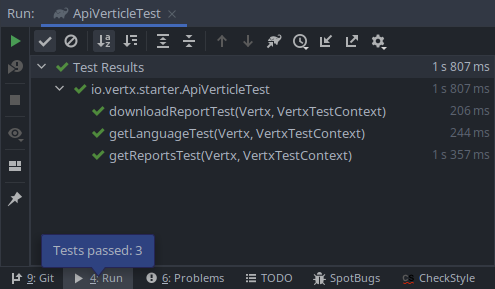
\includegraphics[width=100mm]{img/general/test_api.png}
    \label{fig:api_test}
\end{figure}

\paragraph{AuthVerticleTest}\mbox{}\\
Si tratta di test relativi al servizio di autenticazione, pertanto uno dei componenti principali da testare per permettere l'interazione tra utenti e sistema. In questa classe per il primo test si verifica che un'operazione di sign up vada a buon fine immettendo un nuovo utente nel sistema. Si crea un oggetto JSon con nome utente e password e tramite la route di autenticazione si fa la registrazione, verificando che lo status code corrisponda a 201 e che il corpo della risposta non sia vuoto. \newline

\noindent Il test successivo prevede l'immissione delle stesse credenziali allo scopo di testare il corretto comportamento nel caso di utente già registrato, pertanto questa volta ci si aspetta un messaggio di errore e l'impossibilità di eseguire l'operazione. \newline

\noindent Dopo aver testato la corretta esecuzione della sign up si verifica l'operazione di log in, utilizzando l'utente creato in precedenza e verificando che lo status equivalga a 200 quando si effettua l'accesso. Anche in questo caso, testiamo il suo corretto funzionamento nel caso in cui l'utente immettesse una password errata e ci aspettiamo uno status code di 401.

\begin{figure}[H]
    \caption{Risultati dei Test su AuthVerticle}
    \centering
    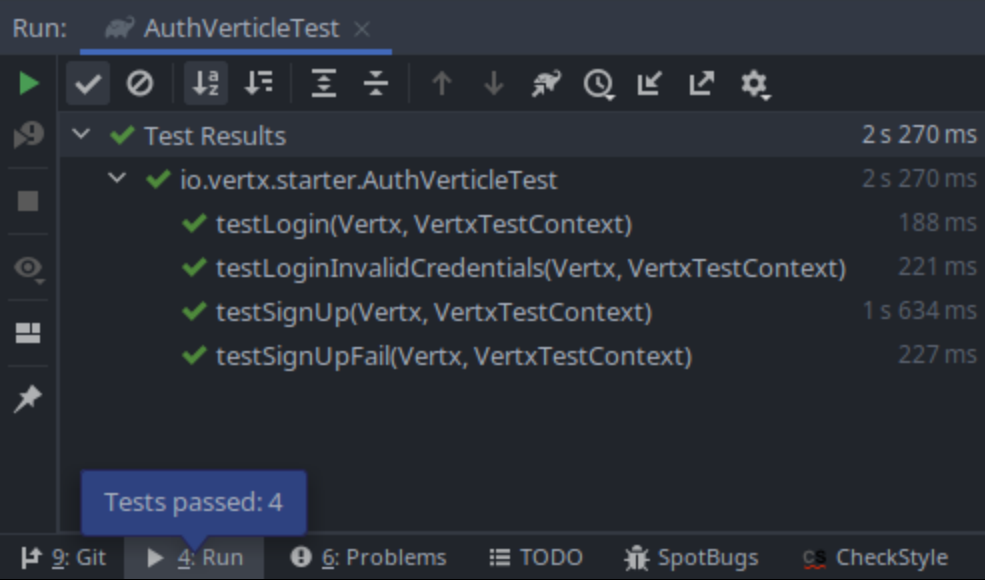
\includegraphics[width=100mm]{img/general/test_auth.png}
    \label{fig:test_auth}
\end{figure}

\paragraph{GameDataStoreVerticleTest}\mbox{}\\
Nella classe GameDataStoreVerticleTest si testano contemporaneamente vari comportamenti, in questo caso si crea inizialmente un report d'esempio e un oggetto JSon che simula un record del database che racchiude i dati di una partita e che racchiude il riferimento a tale report. Successivamente si instanzia un web client e si effettua una post sulla route di game store, aspettandosi uno status code di 201, un corpo di risposta non vuoto e una risposta affermativa dal sistema che ci comunica che l'operazione è andata a buon fine.
\begin{figure}[H]
    \caption{Risultati dei Test su GameDatStoreVerticle}
    \centering
    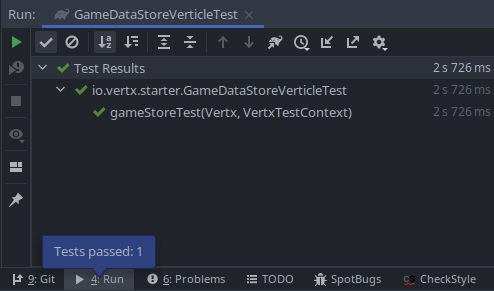
\includegraphics[width=100mm]{img/general/test_store.png}
    \label{fig:test_store}
\end{figure}
\subsection{Ulteriori Strumenti di Test}

\subsubsection{Redux DevTools}
I browser più famosi mettono a disposizione un'estesione per il controllo degli stati di Redux in tempo reale.
Redux DevTools è l'estensione utilizzata per il debug e i test degli stati.\newline
In realtà è possibile utilizzare Redux DevTools con qualsiasi altra architettura che utilizza gli stati ~\cite{ReduxDev96:online}.
\begin{figure}[H]
    \caption{Finestra di Redux Devtool ~\cite{zalmoxis63:online}}
    \centering
    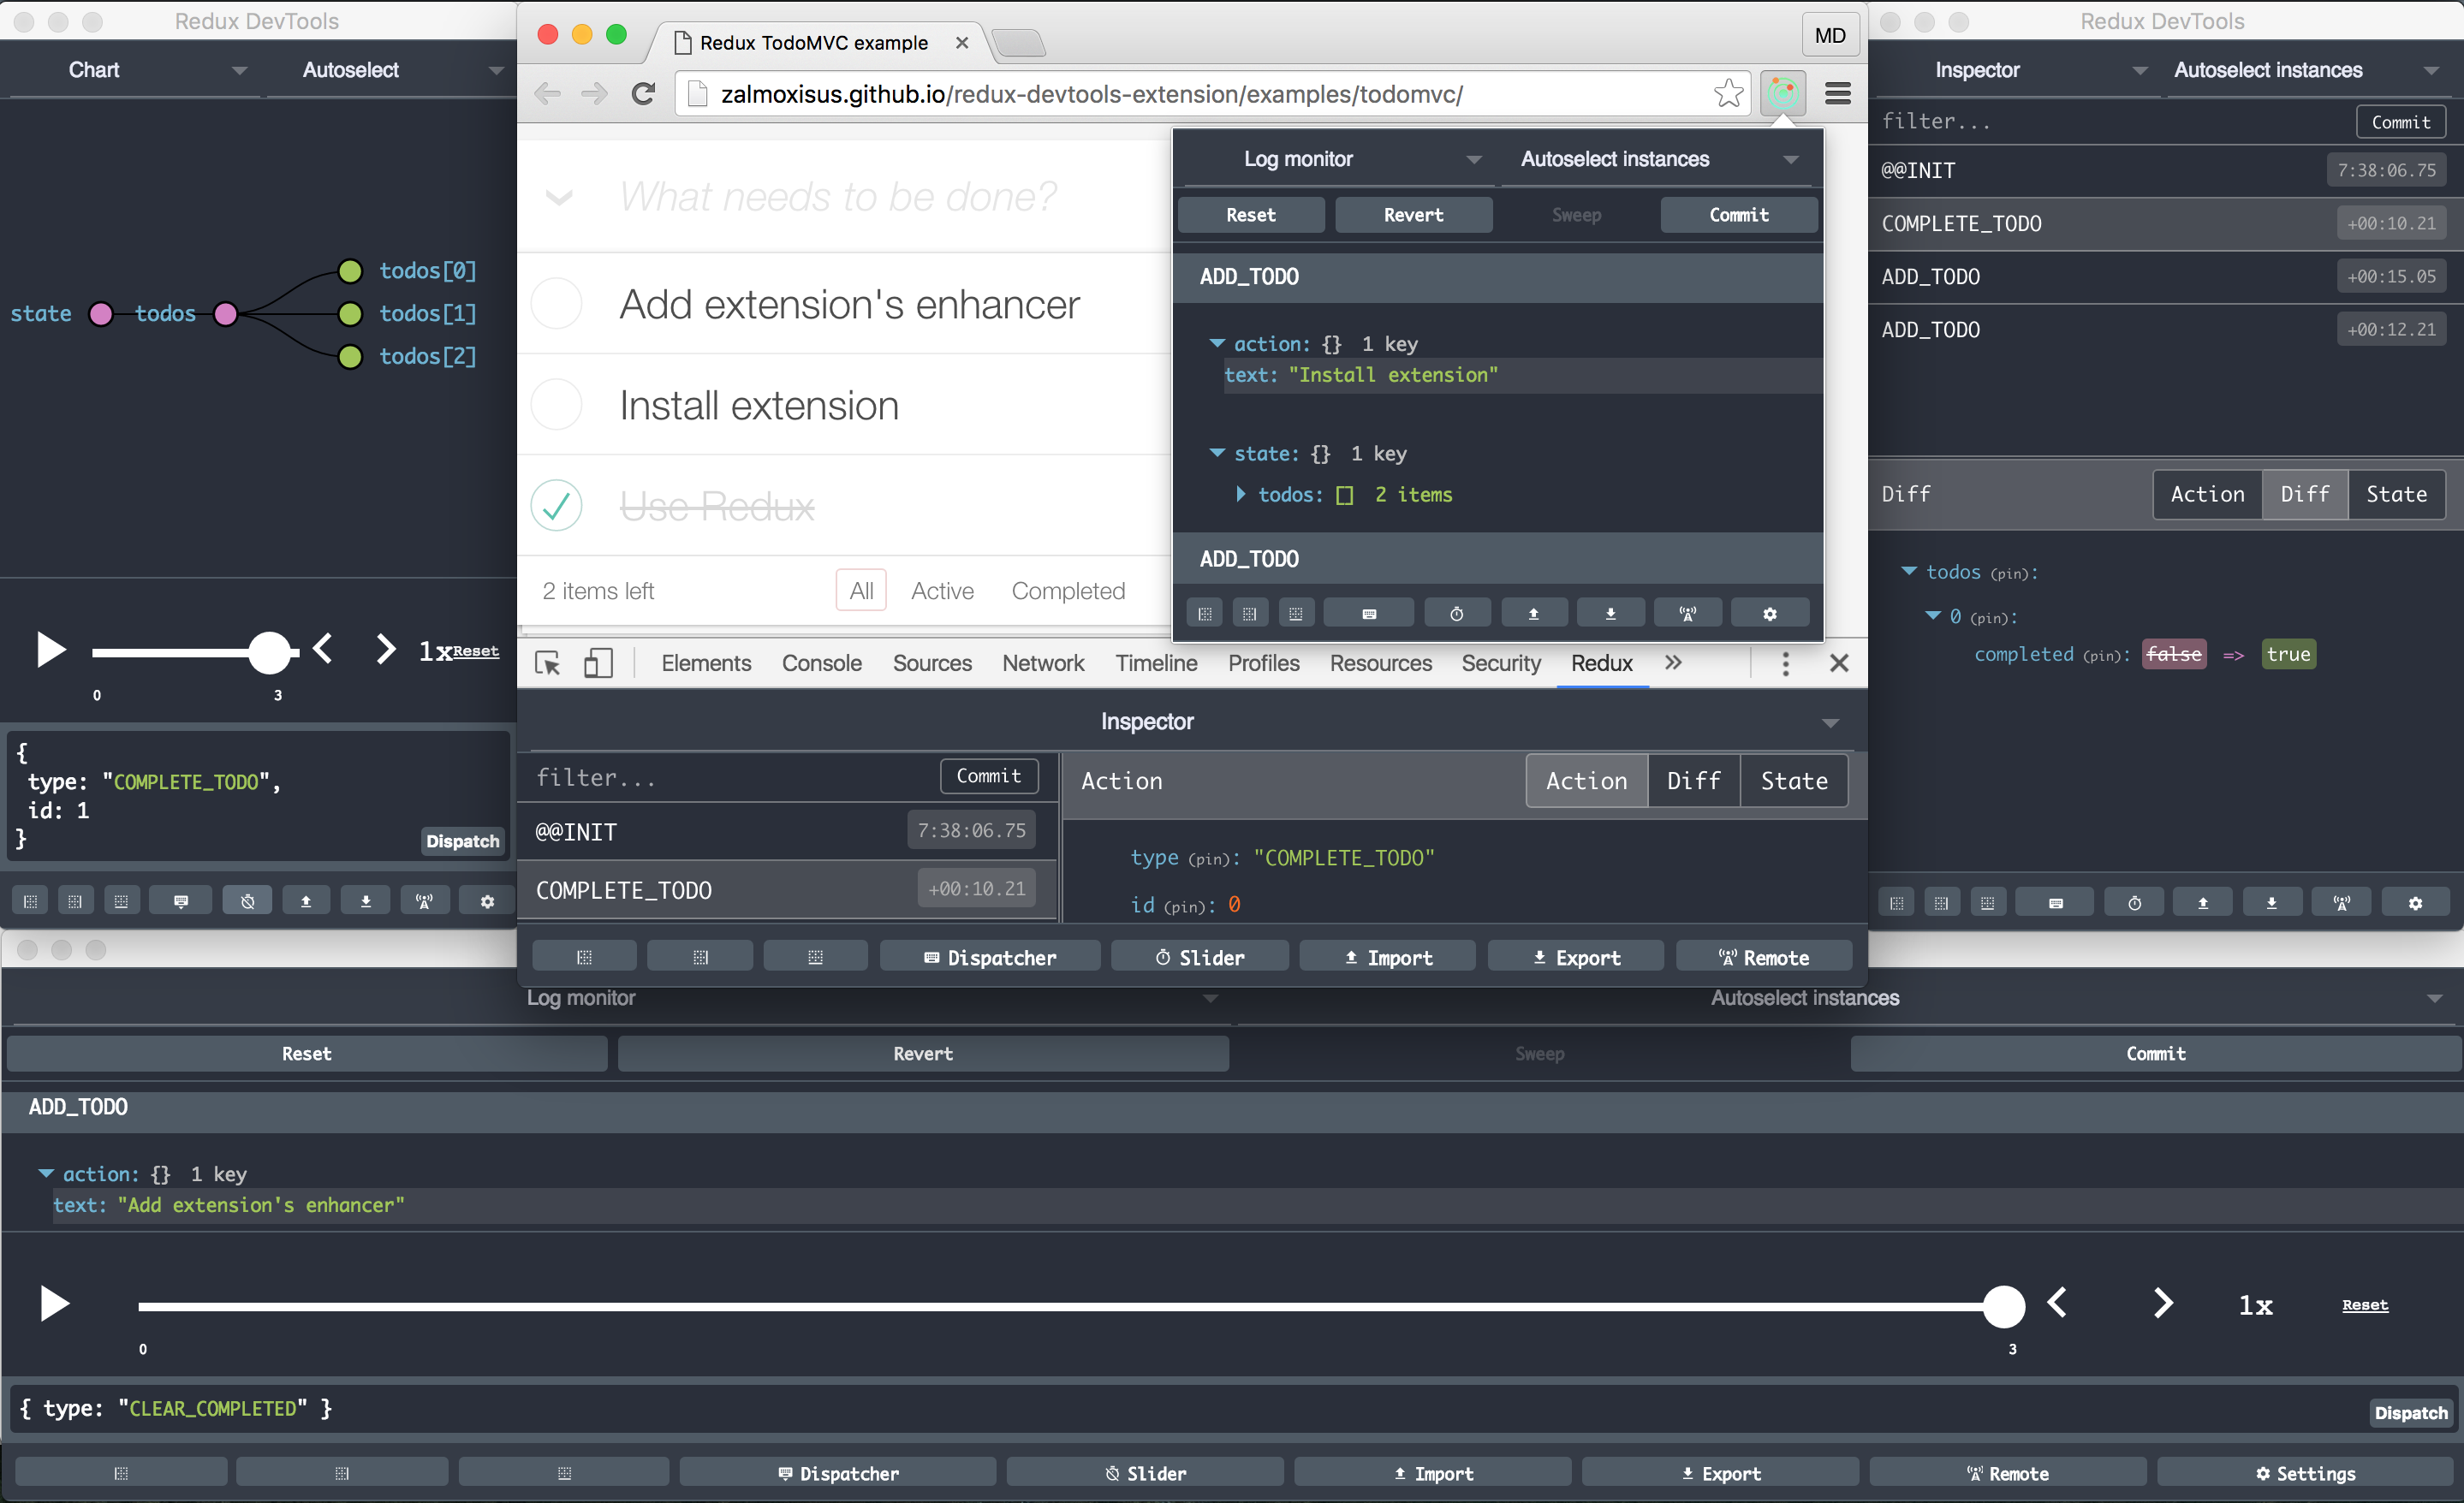
\includegraphics[width=150mm]{img/general/redux_screen.png}
    \label{fig:reduxDevWindow}
\end{figure}
Il progetto open-source è consultabile su GitHub ~\cite{zalmoxis63:online}.

\noindent Redux DevTools è stato utilizzato soprattutto per testare il corretto funzionamento di comunicazione tramite WebSocket.
\begin{figure}[H]
    \caption{Logo di Redux DevTools ~\cite{ReduxDev39:online}}
    \centering
    
\includegraphics[width=30mm]{img/logos/redux_devtool.jpg}
    \label{fig:reduxDev}
\end{figure}
\newpage
